\documentclass[11pt,openany]{report}

\usepackage[a4paper,top=2.45cm,bottom=2.45cm,left=2.55cm,right=2.55cm,headheight=15pt]{geometry}
\usepackage{fontspec}
\setmainfont{Times New Roman}
\setsansfont{Arial}
\setmonofont{Consolas}

\usepackage{amsmath,amssymb,bm}
\usepackage{booktabs,longtable,tabularx,array,multirow}
\usepackage{graphicx}
\usepackage{caption,subcaption,float,placeins}
\usepackage{xcolor}
\usepackage{enumitem}
\usepackage{listings}
\usepackage{fancyhdr,lastpage}
\usepackage{tikz}
\usetikzlibrary{arrows.meta,positioning,calc,shapes.geometric,fit,backgrounds}
\usepackage[hidelinks,unicode]{hyperref}
\usepackage[nameinlink,noabbrev]{cleveref}

\definecolor{ReportBlue}{HTML}{2457A6}
\definecolor{ReportOrange}{HTML}{D9782D}
\definecolor{ReportGold}{HTML}{B28A20}
\definecolor{ReportPink}{HTML}{B44D73}
\definecolor{ReportInk}{HTML}{252A34}
\definecolor{ReportGrey}{HTML}{6B7280}
\definecolor{ReportLight}{HTML}{EEF3FA}
\definecolor{ReportWarm}{HTML}{FFF7ED}

\graphicspath{{figures/}}
\captionsetup{font=small,labelfont=bf,labelsep=quad}
\setlength{\parindent}{1.5em}
\setlength{\parskip}{0.35em}
\setlength{\emergencystretch}{3em}
\renewcommand{\arraystretch}{1.23}
\pagestyle{fancy}
\fancyhf{}
\fancyhead[L]{\small Fixed-Focal 650 nm Posterior-Pole Illumination Simulation}
\fancyfoot[C]{Page \thepage}

\lstdefinestyle{workflow}{basicstyle=\ttfamily\small,backgroundcolor=\color{ReportLight},frame=single,rulecolor=\color{ReportBlue!45},breaklines=true,columns=fullflexible,showstringspaces=false,xleftmargin=1em,xrightmargin=1em}
\lstset{style=workflow}

\newcommand{\D}{\,\mathrm{D}}
\newcommand{\mm}{\,\mathrm{mm}}
\newcommand{\um}{\,\mu\mathrm{m}}
\newcommand{\sourcefile}[1]{\nolinkurl{#1}}
\newcommand{\keyresult}[1]{\textcolor{ReportBlue}{\textbf{#1}}}
\input{generated_results_en.tex}

\title{Fixed-Focal 650 nm Posterior-Pole Illumination\\Optical Simulation Report}
\author{Fixed-Parameter ABCD Model and Ansys Zemax OpticStudio ZOS-API Cross-Validation}
\date{19 August 2026\quad Report version 3.1.0}

\begin{document}
\pagenumbering{Roman}

\begin{titlepage}
  \centering
  \vspace*{1.8cm}
  {\Huge\bfseries Fixed-Focal 650 nm Posterior-Pole Illumination\par}
  \vspace{0.4cm}
  {\Huge\bfseries Optical Simulation Report\par}
  \vspace{0.9cm}
  {\Large Known posterior-pole parameters, three discrete focal lengths, and 60--120 D object-side demands\par}
  \vspace{1.2cm}
  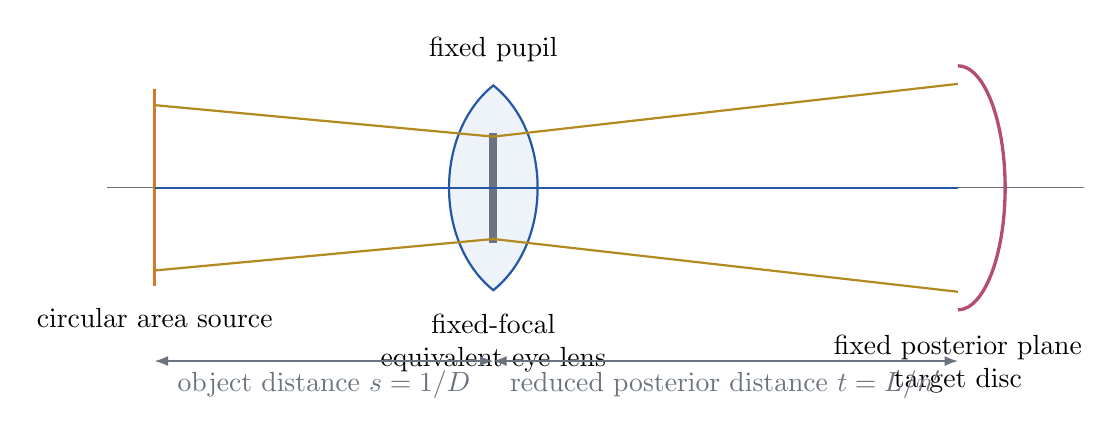
\begin{tikzpicture}[x=1cm,y=1cm,>=Latex]
    \draw[ReportGrey,thin] (-6.2,0)--(6.2,0);
    \draw[ReportOrange,very thick] (-5.6,-1.25)--(-5.6,1.25);
    \node[below] at (-5.6,-1.4) {circular area source};
    \draw[ReportBlue,fill=ReportLight,thick] (-1.3,-1.3) .. controls (-0.55,-0.7) and (-0.55,0.7) .. (-1.3,1.3) .. controls (-2.05,0.7) and (-2.05,-0.7) .. cycle;
    \node[below,align=center] at (-1.3,-1.48) {fixed-focal\\equivalent eye lens};
    \draw[ReportGrey,line width=3pt] (-1.3,-0.7)--(-1.3,0.7);
    \node[above] at (-1.3,1.48) {fixed pupil};
    \draw[ReportPink,very thick] (4.6,-1.55) arc[start angle=-90,end angle=90,x radius=0.6,y radius=1.55];
    \node[below,align=center] at (4.6,-1.75) {fixed posterior plane\\target disc};
    \draw[ReportGold,thick] (-5.6,1.05)--(-1.3,0.65)--(4.6,1.32);
    \draw[ReportBlue,thick] (-5.6,0)--(-1.3,0)--(4.6,0);
    \draw[ReportGold,thick] (-5.6,-1.05)--(-1.3,-0.65)--(4.6,-1.32);
    \draw[<->,ReportGrey] (-5.6,-2.2)--node[below]{object distance $s=1/D$}(-1.3,-2.2);
    \draw[<->,ReportGrey] (-1.3,-2.2)--node[below]{reduced posterior distance $t=L/n'$}(4.6,-2.2);
  \end{tikzpicture}
  \vfill
  {\large Technical report | English edition | A4 | paired Chinese edition\par}
  \vspace{0.25cm}
  {\large 19 August 2026\par}
\end{titlepage}

\chapter*{Technical summary}
\addcontentsline{toc}{chapter}{Technical summary}
\keyresult{The audit has two distinct verdicts: the calculation passes within the declared paraxial model, while the real-experiment status remains NOT READY.} Units, closed-form ABCD coefficients, source diameters, areas, and coverage margins were independently recomputed for all 252 cases. OpticStudio 24.1 Paraxial systems reproduced the same bounds to numerical-rounding precision. This verifies implementation of the first-order equivalent-eye model; it does not validate a real biological eye, absolute irradiance, optical safety, or a biological outcome.

The quantitative applicability screen shows that the maximum conservative source-edge--pupil-edge ray angle exceeds the project's $10^\circ$ real-ray review threshold in all \CasesAboveAngleScreen{} cases, spanning \MinimumEdgeAngle$^\circ$--\MaximumEdgeAngle$^\circ$. In addition, \CasesBelowFfour{} cases have a working F-number below 4. The reported source dimensions are therefore \keyresult{first-order mechanical candidates for subsequent real-surface modelling and bench calibration}, not final source-size, power, or exposure prescriptions for human or animal studies.

This version corrects the principal assumption of the earlier model. That model changed the chick or human equivalent focal length continuously so that every object distance met an exact focus condition. It consequently treated the 60--120 D object-side demands as ocular accommodation demands and reported that every case exceeded an accommodation limit. The corrected model uses \keyresult{only three discrete fixed focal lengths for each eye, fixes the posterior plane from the known axial parameter, and treats object distance, focal length, and pupil as independent inputs.}

The fixed focal lengths are the two endpoints and arithmetic midpoint of each PPT range:
\begin{itemize}[leftmargin=2.2em,noitemsep]
  \item chick: $7.5\mm$, $8.0\mm$, and $8.5\mm$;
  \item child: $13.5\mm$, $15.1\mm$, and $16.7\mm$;
  \item adult: $12.8\mm$, $14.75\mm$, and $16.7\mm$.
\end{itemize}
Object-side demand remains $60,70,80,90,100,110,120\D$, and four pupil diameters are scanned for each eye. The main matrix contains
\[
3\text{ eyes}\times3\text{ fixed focal lengths}\times4\text{ pupils}\times7\text{ object distances}
=\keyresult{\MainSweepRows\text{ cases}}.
\]
Each row reports a geometric minimum source diameter and a conservative full-overlap source diameter. The former makes the outer support of the footprint reach the target; the latter keeps the complete posterior target inside the full-overlap plateau of the source-image and pupil-footprint convolution. The latter is useful as an initial mechanical-space candidate, but it is not an experiment-release value before real-surface, radiometric, and safety calibration.

For the adult eye at $f=16.7\mm$ and its maximum pupil, the conservative diameters at $60\D$ and $120\D$ are \keyresult{\AdultSixtyConservative\,mm} and \keyresult{\AdultOneTwentyConservative\,mm}. For the chick at $f=8.5\mm$, the corresponding values are \keyresult{\ChickSixtyConservative\,mm} and \keyresult{\ChickOneTwentyConservative\,mm}. None of these values is released for live exposure.

Six fixed-focal Paraxial systems were built through the ZOS-API in OpticStudio 24.1. The maximum difference between the analytical and traced footprint bounds was \keyresult{$\ZosMaxError\um$}. This establishes agreement between the fixed-parameter ABCD implementation and Zemax first-order propagation, not agreement with real-eye aberration, scattering, absolute irradiance, or optical safety.

\tableofcontents
\clearpage
\pagenumbering{arabic}

\chapter{Corrected question and applicability verdict}

\section{The old conclusion failed because it forced focus, not because the object distance was inherently impossible}
The previous model solved a new ocular power for every object distance so that the total transfer matrix satisfied the imaging condition $B_m=0$. When the baseline image distance was also calibrated as $t=1/F_0$, the no-external-lens case collapsed to ``added optical power equals object-side demand.'' The 60--120 D range was therefore interpreted as 60--120 D of accommodation and compared with a physiological accommodation limit. That calculation answered whether the eye could change focal length continuously to image the object plane sharply at the posterior pole. It did not answer the actual design question: how large the source must be to cover the posterior target when focal length and posterior parameters are fixed.

\section{The corrected model fixes focal length and posterior location while external conditions change}
Each discrete focal length is run as its own experiment. Within one case, focal length $f$, axial length $L$, posterior target diameter, pupil, and object distance are known. The solver is not allowed to infer a new $f$. Outputs are limited to source-plane size, mapping coefficients, pupil footprint, geometric coverage margin, and conservative full-overlap margin. Accommodation-limit language is no longer used as a main-sweep verdict.

\section{The first-order candidate is the full-overlap diameter, not the geometric minimum}
The geometric minimum can be zero when the fixed-focal pupil-defocus footprint already extends to the posterior target edge. This occurs in \GeometricZeroCount{} of the \MainSweepRows{} cases. Zero does not describe an installable zero-area source and does not guarantee minimum edge irradiance. The conservative diameter is always positive and places the entire target within the full-overlap region. It is better suited to subsequent real-ray, irradiance-threshold, scattering, and safety work, but it is still not a live-experiment setting.

\chapter{Inputs and fixed-focal definitions}

\section{Eye parameters from the source PPT}
\begin{table}[H]
\centering
\caption{Fixed posterior parameters and three discrete focal lengths}
\begingroup
\small
\setlength{\tabcolsep}{4pt}
\begin{tabularx}{\textwidth}{>{\raggedright\arraybackslash}p{3.0cm}>{\centering\arraybackslash}p{2.0cm}>{\centering\arraybackslash}p{2.0cm}>{\centering\arraybackslash}p{2.0cm}>{\raggedright\arraybackslash}X}
\toprule
Model & Axial length (mm) & Target diameter (mm) & Maximum pupil (mm) & Fixed focal lengths (mm)\\
\midrule
\FocalRows
\bottomrule
\end{tabularx}
\endgroup
\end{table}

The chick model uses an $11.7\mm$ axial length and a $3\mm$ posterior target. Child and adult models use axial lengths of $23.0\mm$ and $23.6\mm$, respectively, with $6\mm$ posterior targets. Four pupil levels discretize the PPT range for each eye. The longest and shortest focal lengths are the PPT range endpoints; the middle value is the arithmetic midpoint, not a fitted result.

\section{Object-side demand and object distance}
Positive demand denotes the magnitude of inverse object distance:
\[
D=\frac{1}{s},\qquad s=\frac{1}{D}.
\]
$60\D$ corresponds to $16.667\mm$, and $120\D$ corresponds to $8.333\mm$. These quantities describe the geometric separation between the source plane and the equivalent-eye lens. They are not accommodation demands.

\section{The posterior plane uses a fixed reduced distance}
The ray state is $[y,n\theta]^\mathsf{T}$. Propagation in the image medium uses $n'=1.336$, giving
\[
t=\frac{L}{n'}.
\]
This maps the full axial length from the PPT into reduced-angle ABCD coordinates. It is more consistent with the requirement for a known, fixed posterior parameter than imposing $t=1/F$. The equivalent principal-plane location nevertheless remains a model quantity that must be measured or calibrated with an anatomical model in the next stage.

\chapter{Fixed-parameter ABCD model}

\section{Lens and propagation matrices}
Air propagation and fixed eye power are
\[
T(s)=\begin{bmatrix}1&s\\0&1\end{bmatrix},\qquad
L(P)=\begin{bmatrix}1&0\\-P&1\end{bmatrix},\qquad P=\frac{1}{f}.
\]
The complete matrix is
\[
M=T(t)L(P)T(s).
\]
Unlike the earlier model, the corrected model does not solve for $P$; it is limited to one of the three configured values.

\section{Independent source and pupil mappings}
For source-plane height $y_s$ and pupil height $y_p$, the posterior height is
\[
y_r=m_s y_s+m_p y_p,
\]
where
\[
m_s=-\frac{t}{s},\qquad m_p=1+\frac{t}{s}-tP.
\]
$m_s$ maps source-plane dimensions to the posterior pole. $m_p$ describes the defocus footprint formed by a finite pupil when fixed focal length and fixed object distance do not match an exact focus. Pupil and fixed focal length therefore affect the result explicitly.

\section{Two source-size definitions}
Let posterior-target radius be $R_t$, pupil radius $R_p$, and source radius $R_s$, and define
\[
a=|m_s|,\qquad b=|m_p|R_p.
\]
The mapped source disc and pupil disc form a convolution footprint. Its outer-support radius is $aR_s+b$, and its full-overlap plateau radius is $aR_s-b$. Thus
\begin{align}
R_{s,\mathrm{geo}}&=\frac{\max(0,R_t-b)}{a},\\
R_{s,\mathrm{cons}}&=\frac{R_t+b}{a}.
\end{align}
The geometric minimum makes the outer support reach the target. The conservative radius makes the full-overlap plateau cover the target. Both follow directly from fixed parameters and require no focal-length iteration.

\begin{figure}[H]
\centering
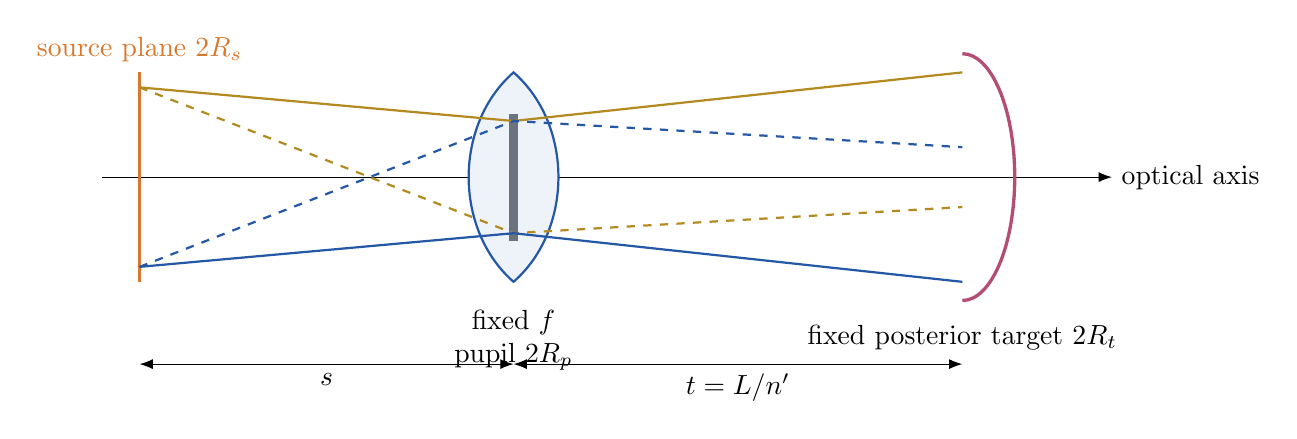
\begin{tikzpicture}[scale=0.95,>=Latex]
  \draw[->] (-0.5,0)--(13,0) node[right]{optical axis};
  \draw[ReportOrange,very thick] (0,-1.4)--(0,1.4) node[above]{source plane $2R_s$};
  \draw[ReportBlue,fill=ReportLight,thick] (5,-1.4) .. controls (5.8,-0.7) and (5.8,0.7) .. (5,1.4) .. controls (4.2,0.7) and (4.2,-0.7) .. cycle;
  \draw[ReportGrey,line width=3pt] (5,-0.85)--(5,0.85);
  \node[below,align=center] at (5,-1.65){fixed $f$\\pupil $2R_p$};
  \draw[ReportPink,very thick] (11,-1.65) arc[start angle=-90,end angle=90,x radius=0.7,y radius=1.65];
  \node[below] at (11,-1.85){fixed posterior target $2R_t$};
  \draw[ReportGold,thick] (0,1.2)--(5,0.75)--(11,1.4);
  \draw[ReportGold,dashed,thick] (0,1.2)--(5,-0.75)--(11,-0.4);
  \draw[ReportBlue,thick] (0,-1.2)--(5,-0.75)--(11,-1.4);
  \draw[ReportBlue,dashed,thick] (0,-1.2)--(5,0.75)--(11,0.4);
  \draw[<->] (0,-2.5)--node[below]{$s$}(5,-2.5);
  \draw[<->] (5,-2.5)--node[below]{$t=L/n'$}(11,-2.5);
\end{tikzpicture}
\caption{Ray mapping with fixed focal length, fixed pupil, and fixed posterior plane. Solid and dashed rays are different source-edge and pupil-edge combinations.}
\end{figure}

\chapter{Experiment matrix and reproducible workflow}

\section{Complete experiment design}
The main sweep contains:
\begin{itemize}[leftmargin=2.2em]
  \item eye model: 30--45-day-old chick, 6-year-old child, and 18-year-old adult;
  \item fixed focal length: three discrete values for each eye;
  \item object-side demand: $60$--$120\D$ in $10\D$ increments;
  \item pupil: four diameters for each eye;
  \item posterior pole: axial length and target diameter fixed by the model;
  \item outputs: mapping coefficients, defocus footprint, geometric and conservative source diameters/areas, and coverage margins.
\end{itemize}
The external negative lens is excluded from the main matrix. The PPT defines it as a later experiment after the baseline models are established. Actual vertex distance and component order should be confirmed before adding that factor.

\section{Automated workflow}
\begin{figure}[H]
\centering
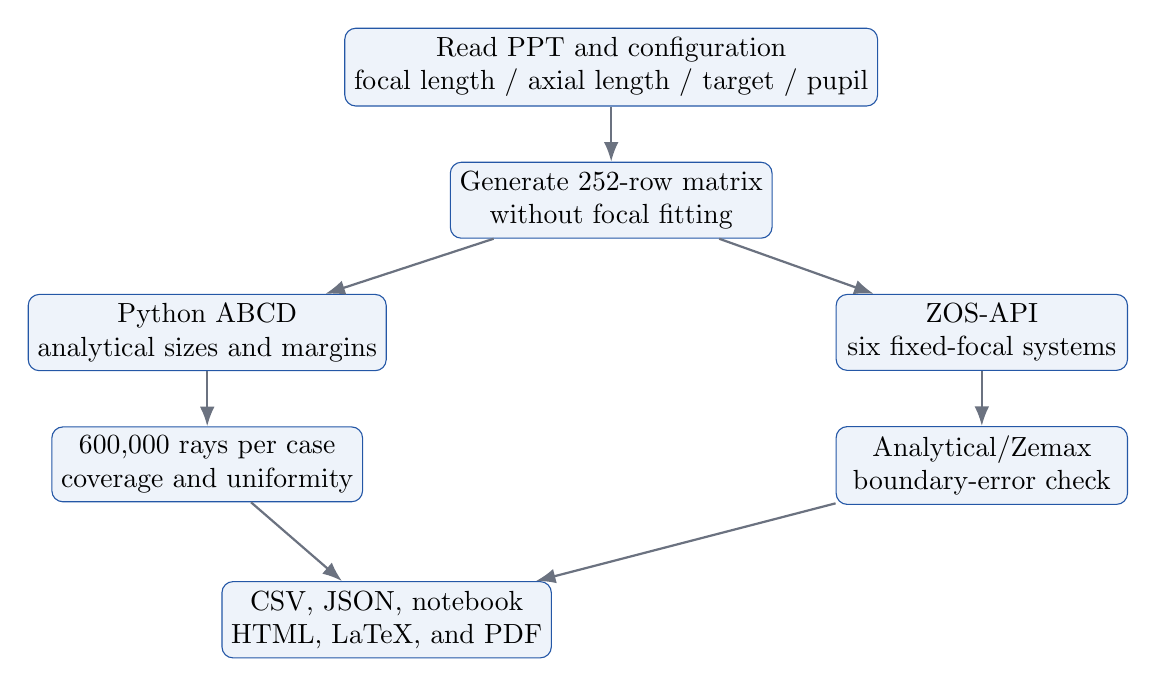
\begin{tikzpicture}[node distance=7mm and 8mm,box/.style={draw=ReportBlue,rounded corners,fill=ReportLight,align=center,minimum width=3.7cm,minimum height=0.9cm},arrow/.style={-{Latex[length=2.5mm]},thick,ReportGrey}]
  \node[box] (ppt) {Read PPT and configuration\\focal length / axial length / target / pupil};
  \node[box,below=of ppt] (matrix) {Generate 252-row matrix\\without focal fitting};
  \node[box,below left=of matrix] (abcd) {Python ABCD\\analytical sizes and margins};
  \node[box,below right=of matrix] (zos) {ZOS-API\\six fixed-focal systems};
  \node[box,below=of abcd] (mc) {600,000 rays per case\\coverage and uniformity};
  \node[box,below=of zos] (cross) {Analytical/Zemax\\boundary-error check};
  \node[box,below right=10mm and -18mm of mc] (artifacts) {CSV, JSON, notebook\\HTML, LaTeX, and PDF};
  \draw[arrow] (ppt)--(matrix);
  \draw[arrow] (matrix)--(abcd);
  \draw[arrow] (matrix)--(zos);
  \draw[arrow] (abcd)--(mc);
  \draw[arrow] (zos)--(cross);
  \draw[arrow] (mc)--(artifacts);
  \draw[arrow] (cross)--(artifacts);
\end{tikzpicture}
\caption{Reproducible workflow from fixed inputs to auditable report artifacts.}
\end{figure}

\section{One-command reproduction}
\begin{lstlisting}
powershell -ExecutionPolicy Bypass -File `
  experiments/eye_illumination/run_all.ps1 `
  -PythonPath <python.exe> `
  -OpticStudioDir "C:\Program Files\Ansys Zemax OpticStudio 2024 R1.00"

powershell -ExecutionPolicy Bypass -File `
  experiments/eye_illumination/report/latex/build_report.ps1 `
  -PythonPath <python.exe>
\end{lstlisting}
The first command regenerates the main sweep, Monte Carlo analysis, Zemax systems, cross-validation, notebook, and HTML report. The second regenerates Chinese and English charts, both XeLaTeX PDFs, and the PDF QA records.

\chapter{Fixed-focal source-size results}

\section{Three discrete focal lengths create distinct design curves}
\begin{figure}[H]
\centering
\includegraphics[width=0.98\textwidth]{source_diameter_en.png}
\caption{Conservative source diameter for the three fixed focal lengths at the maximum pupil of each eye. The horizontal axis is object-side demand, not accommodation demand.}
\label{fig:source-en}
\end{figure}
Every line in \cref{fig:source-en} retains one focal length from start to finish. The nontrivial shape reflects competing changes: shorter object distance increases the source-to-posterior mapping scale $|m_s|$, while the fixed-focal pupil footprint $|m_p|R_p$ also changes. The corrected model no longer produces the old pattern in which all eye types were nearly identical and the source size exactly halved between 60 D and 120 D.

\section{Exact endpoint lookup values}
\begingroup
\small
\setlength{\tabcolsep}{3.2pt}
\begin{longtable}{p{2.75cm}*{6}{>{\centering\arraybackslash}p{1.55cm}}}
\caption{Geometric-minimum and conservative source diameters at 60 D and 120 D for the maximum pupil (mm)}\\
\toprule
Model & $f$ & Pupil & 60 D geo. & 60 D cons. & 120 D geo. & 120 D cons.\\
\midrule
\endfirsthead
\toprule
Model & $f$ & Pupil & 60 D geo. & 60 D cons. & 120 D geo. & 120 D cons.\\
\midrule
\endhead
\EndpointRows
\bottomrule
\end{longtable}
\endgroup
Some 120 D geometric minima are zero because the pupil-defocus footprint reaches or exceeds the target edge. The conservative column is the appropriate first-order mechanical candidate. A smaller value between the geometric and conservative definitions may become acceptable only after a real-surface non-sequential irradiance simulation applies a defined minimum-irradiance criterion. Neither column is a live-exposure prescription without that evidence.

\section{Pupil is an explicit design variable}
\begin{figure}[H]
\centering
\includegraphics[width=0.9\textwidth]{fixed_focal_pupil_en.png}
\caption{Joint influence of pupil and fixed focal length on conservative source size for adult-eye endpoint cases at 60 D and 120 D.}
\label{fig:pupil-en}
\end{figure}
\Cref{fig:pupil-en} shows why one maximum-pupil result cannot represent every pupil state. Conservative size increases with the pupil footprint because the target must remain in the full-overlap plateau. The geometric minimum may instead decrease as the pupil grows. These opposing trends make the acceptance definition essential.

\section{Independent defocus-footprint sensitivity}
\begin{figure}[H]
\centering
\includegraphics[width=0.96\textwidth]{defocus_blur_en.png}
\caption{Equivalent defocus footprint at the fixed image plane for different pupils; dashed lines are posterior-target diameters.}
\end{figure}
This figure explains the physical role of $m_p$; it does not ask the eye to accommodate. A larger defocus footprint can help outer-boundary coverage but reduces spatial selectivity and the fraction of rays used inside the target. Source size, minimum irradiance, and optical safety must therefore be evaluated together.

\chapter{Monte Carlo and OpticStudio validation}

\section{Geometric-minimum and conservative designs have different irradiance shapes}
\begin{figure}[H]
\centering
\includegraphics[width=0.92\textwidth]{monte_carlo_en.png}
\caption{Adult eye, $f=16.7\mm$, 5 mm pupil, 60 D; 600,000 deterministic pseudo-random rays per design. The white circle is the 6 mm posterior target.}
\label{fig:mc-en}
\end{figure}
The geometric-minimum design captures \GeometricCapture\% of its rays in the target and has a target p10-to-mean uniformity ratio of \GeometricUniformity. The conservative design gives \ConservativeCapture\% and \ConservativeUniformity, respectively. The larger conservative source can send more rays outside the target, reducing capture fraction, while substantially reducing edge roll-off inside the target. Coverage and optical efficiency are not the same metric.

\section{ZOS-API validates the fixed-parameter footprint boundary}
\begin{figure}[H]
\centering
\includegraphics[width=0.88\textwidth]{zos_validation_en.png}
\caption{Analytical and OpticStudio upper bounds for fixed-focal retinal ray height.}
\end{figure}
\begingroup
\scriptsize
\setlength{\tabcolsep}{3pt}
\begin{longtable}{p{4.0cm}*{5}{>{\centering\arraybackslash}p{1.65cm}}}
\caption{Six fixed-focal OpticStudio cross-validation systems}\\
\toprule
Case & $f$ (mm) & Object distance (mm) & Pupil (mm) & Conservative diameter (mm) & Boundary error ($\mu$m)\\
\midrule
\endfirsthead
\toprule
Case & $f$ (mm) & Object distance (mm) & Pupil (mm) & Conservative diameter (mm) & Boundary error ($\mu$m)\\
\midrule
\endhead
\ZosRows
\bottomrule
\end{longtable}
\endgroup
Each system writes equivalent-eye focal length, object distance, pupil, and reduced posterior distance into a sequential Paraxial system. Positive and negative source edges combined with positive and negative pupil edges form four corner rays. The maximum boundary error of \ZosMaxError\,$\mu$m is at numerical-rounding scale, confirming that the Python matrix and OpticStudio use the same fixed-parameter propagation relation.

\section{Automated quality controls}
Validation requires exactly seven object-side demands in 10 D increments; three configured focal lengths and four pupils per eye; 252 unique rows; no accommodation output column; conservative diameter no smaller than the geometric minimum; full-overlap residual below $10^{-8}\um$; six saved ZOS systems with a valid API license; and analytical/Zemax boundary error below $10^{-6}\um$. A separate script that does not call production model functions recomputes $s$, $m_s$, $m_p$, source diameters, areas, maximum edge angle, and F-number from the CSV. Numerical failure stops the reproducible workflow. Real-experiment readiness remains a separate blocked state and never changes automatically because a mathematical test passes.

\chapter{Limitations, uncertainty, and next modelling stage}

\section{Applicability diagnostics block direct live-experiment use}
\begin{figure}[H]
\centering
\includegraphics[width=0.98\textwidth]{model_applicability_en.png}
\caption{Paraxial-applicability screen for all 252 cases. The $10^\circ$ line is a conservative project trigger for real-ray review, not a universal certificate. The F/4 reference follows OpticStudio guidance on OPD accuracy for a Paraxial surface.}
\label{fig:applicability-en}
\end{figure}
\Cref{fig:applicability-en} shows that the maximum edge angle exceeds $10^\circ$ in all \CasesAboveAngleScreen{} cases and exceeds $15^\circ$ in all \CasesAboveFifteen{} cases. \CasesBelowFfour{} cases are faster than F/4, and \CasesPassingBothScreens{} cases pass both project screens. \href{https://ansyshelp.ansys.com/public/Views/Secured/Zemax/v252/en/OpticStudio_User_Guide/OpticStudio_Help/topics/Paraxial_and_Parabasal_Rays.html}{Ansys documentation on paraxial rays} explicitly depends on small-angle linearization. Its \href{https://ansyshelp.ansys.com/public/Views/Secured/Zemax/v25101/en/OpticStudio_User_Guide/OpticStudio_Help/topics/Paraxial_sequential_surfaces_lens_data_editor.html}{Paraxial surface documentation} also recommends a working F-number no faster than approximately F/4 for best OPD accuracy. Agreement between two ideal Paraxial implementations cannot reveal real-surface deviations at large angles or fast beams.

\section{The three midpoint focal lengths still require user confirmation}
The user requires only three fixed focal lengths per eye, but the PPT gives a range rather than three measured values. This report uses a transparent endpoint-plus-arithmetic-midpoint rule. If the intended values differ, update the arrays in \sourcefile{config/experiment.json} and rerun; the program rejects focal lengths outside the configured set in baseline mode.

\section{Equivalent principal-plane location remains uncertain}
Using $t=L/1.336$ is an auditable first-order conversion from axial length to reduced posterior distance. A real eye's equivalent principal plane does not coincide with the corneal vertex and depends on the cornea, crystalline lens, aqueous and vitreous indices, and potentially a GRIN lens. The next model should explicitly represent anterior and posterior corneal surfaces, lens/GRIN, refractive indices, and retinal curvature, then calibrate the image plane to measured axial length.

\section{Geometric coverage is not irradiance or safety}
The PPT does not specify source radiance, spectral bandwidth, exposure time, tissue transmission, or a safety limit. This report therefore provides relative ray counts and geometry only. Animal or human experiments require traceable absolute-radiometry calibration with measurement uncertainty and a formal retinal thermal and photochemical hazard assessment. Ophthalmic instruments should be evaluated against \href{https://www.iso.org/standard/79919.html}{ISO 15004-2:2024}; incoherent LED/lamp systems against \href{https://webstore.iec.ch/en/publication/7076}{IEC 62471}; and laser systems against \href{https://webstore.iec.ch/en/publication/3587}{IEC 60825-1}, as applicable. Institutional optical-safety specialists must determine applicability and final limits.

\section{Live studies require ethics approval and hardware safety controls}
Chick experiments involve live vertebrate animals and require the applicable animal ethics or IACUC-equivalent approval, veterinary oversight, fixation/anesthesia rules, monitoring, stopping criteria, and post-procedure observation. Human studies require applicable IRB/ethics approval and informed consent. Both require approved hardware power limits, interlocks, exposure timers, fail-safe behavior, and independent power verification. Software-derived dimensions do not replace those controls.

\section{Add the external lens only after the fixed-focal baseline is confirmed}
The negative-lens scan in the PPT is a later extension. Confirm the three fixed focal lengths, lens vertex distance, and component order at extremely short object distances before creating a fixed-focal-length $\times$ object-distance $\times$ pupil $\times$ external-lens matrix. Do not restore the earlier approach of changing ocular focal length to compensate for an external lens.

\chapter{Reproducible artifacts and audit path}

\section{Primary data files}
\begin{longtable}{p{5.6cm}p{9.2cm}}
\toprule
File & Contents\\
\midrule
\sourcefile{fixed\_focal\_source\_sweep.csv} & Complete 252-row matrix with fixed focal length, object distance, pupil, mapping coefficients, two source-size definitions, and coverage margins\\
\sourcefile{headline\_results.csv} & 63-row endpoint lookup table at the maximum pupil of each model\\
\sourcefile{monte\_carlo\_summary.json} & Capture and uniformity metrics for 600,000 rays in each source-size definition\\
\sourcefile{zemax/zosapi\_validation.csv} & Analytical/traced boundary comparison for six fixed-focal ZOS systems\\
\sourcefile{validation\_report.json} & Automated verdicts for row count, parameter levels, coverage identities, license state, and ZOS error\\
\sourcefile{real\_experiment\_readiness.json/.md} & Independent closed-form recomputation, angle/F-number screen, source-quality assessment, and real-experiment blockers\\
\sourcefile{eye\_illumination\_analysis.ipynb} & Executed notebook with data, figures, and validation results\\
\bottomrule
\end{longtable}

\section{Version-control strategy}
Configuration, code, CSV, JSON, notebook, Zemax systems, LaTeX sources, figures, and both final PDFs are versioned together. Immutable experiment records store configuration and key-artifact SHA-256 values so later work can distinguish parameter changes, code changes, and presentation-only changes. Large binary files remain under Git LFS. GitHub Actions reruns unit tests and static compilation checks on Windows x64.

\chapter{Conclusions and recommended next steps}
The corrected experiment removes the confusion between object-side demand and accommodation demand. Chick, child, and adult equivalent focal lengths now use three discrete fixed values per model; posterior location is fixed; and object distance, pupil, and focal length jointly determine the source footprint. The main sweep reports auditable geometric-minimum and conservative full-overlap sizes rather than declaring that every case exceeds an accommodation limit.

Independent audit confirms that these dimensions are internally correct within the paraxial model, but \keyresult{the real-experiment status is NOT READY}. Every case exceeds the project $10^\circ$ review trigger, many chick cases use fast beams, and the PPT does not provide a complete anatomical prescription, source radiometry, exposure time, or safety dose. Conservative diameters are suitable only for mechanical-space reservation and the next real model; geometric minima are first-order theoretical lower bounds. The adult $f=16.7\mm$, 5 mm-pupil values of \AdultSixtyConservative\,mm at $60\D$ and \AdultOneTwentyConservative\,mm at $120\D$ must not be used directly for live exposure.

The minimum release path is to obtain individual or reliable anatomical data; build a real-surface eye; rerun with real rays and non-sequential radiometry; validate coverage, uniformity, and absolute irradiance on a physical eye model or calibrated detector; complete ISO/IEC optical-safety assessment; obtain animal or human ethics approval; and only then write approved values with measurement uncertainty and hardware limits into the experimental protocol. \href{https://optics.ansys.com/hc/en-us/articles/42661670424851-Exploring-Non-Sequential-Mode-in-OpticStudio}{Ansys guidance on Non-Sequential Mode} provides the starting point for source, material, and detector modelling.

\appendix
\chapter{Result-field definitions}
\begin{longtable}{p{5.4cm}p{9.4cm}}
\toprule
Field & Definition\\
\midrule
\sourcefile{fixed\_focal\_length\_mm} & Fixed equivalent focal length assigned to the current case; restricted to the three configured baseline values\\
\sourcefile{source\_demand\_D} & Magnitude of inverse object distance $1/s$, not accommodation\\
\sourcefile{reduced\_retina\_distance\_mm} & Reported axial length divided by the image-space refractive index 1.336\\
\sourcefile{source\_mapping\_coefficient} & Linear source-plane-to-posterior height coefficient $m_s$\\
\sourcefile{pupil\_mapping\_coefficient} & Linear pupil-to-posterior height coefficient $m_p$\\
\sourcefile{pupil\_blur\_diameter\_mm} & $2|m_p|R_p$, the pupil-footprint diameter at the fixed posterior plane\\
\sourcefile{geometric\_min\_source\_diameter\_mm} & Theoretical minimum source diameter whose outer support reaches the posterior-target edge\\
\sourcefile{conservative\_source\_diameter\_mm} & Paraxial candidate diameter whose full-overlap plateau covers the entire posterior target; not a live-experiment release value\\
\sourcefile{maximum\_source\_pupil\_ray\_angle\_deg} & Largest geometric angle among four conservative source-edge and pupil-edge combinations, used for small-angle applicability screening\\
\sourcefile{working\_f\_number} & Fixed effective focal length divided by pupil diameter, used to flag fast-beam cases\\
\sourcefile{real\_experiment\_readiness} & Fixed blocked state requiring calibration, preventing first-order values from being presented as experimental release\\
\sourcefile{geometric\_coverage\_margin\_um} & Outer-support margin relative to the target edge\\
\sourcefile{conservative\_plateau\_margin\_um} & Full-overlap plateau margin relative to the target edge; expected to be near zero\\
\bottomrule
\end{longtable}

\chapter{Audit checklist}
\begin{enumerate}[leftmargin=2.2em]
  \item each eye has exactly three fixed focal lengths in the configuration;
  \item the seven 60--120 D object distances are not treated as accommodation;
  \item reduced posterior distance comes from axial length and refractive index rather than the current focal length;
  \item all 252 main-sweep rows are generated;
  \item both coverage definitions have explicit equations and nonnegative margins;
  \item six fixed-focal OpticStudio systems are saved and cross-validated;
  \item the independent audit recomputes closed-form outputs and applicability metrics without production model functions;
  \item software and reports keep real-experiment readiness blocked and never present Paraxial PASS as safety release;
  \item notebook, HTML, LaTeX, PDFs, and result tables share one configuration and evidence base;
  \item Chinese and English PDFs use A4 pages, language-matched figures, and final layout QA.
\end{enumerate}

\end{document}
